\section{گام اول: خواندن و پیش‌پردازش تصاویر (بخش ۰)}

در این بخش هدف ما آماده‌سازی تصاویر ورودی برای پردازش‌های بعدی است. طبق خواسته‌ی تمرین، ابتدا باید تصاویر دو مجموعه را وارد کرده، آن‌ها را از حالت رنگی سه‌کاناله به تک‌کاناله \lr{(Grayscale)} تبدیل کنیم و در نهایت مقادیر آن‌ها را به فرمت \lr{float32} ببریم.

\begin{notebox}
\textbf{تبدیل به \lr{Grayscale}:} پردازش تصاویر رنگی در هرم‌های لاپلاسی \lr{(Laplacian Pyramids)} به دلیل داشتن سه کانال \lr{(R, G, B)} حجم محاسبات را بالا برده و تحلیل فرکانسی را پیچیده می‌کند. بنابراین، تبدیل تصاویر به مقیاس خاکستری، محاسبات را بسیار ساده‌تر می‌سازد.
\end{notebox}

\subsection{پیاده‌سازی مرحله به مرحله}

ابتدا کتابخانه‌های مورد نیاز برای خواندن تصاویر و انجام عملیات ماتریسی را فراخوانی می‌کنیم:

\begin{codebox}[\lr{Imports}]
\begin{lstlisting}[language=Python]
import cv2
import numpy as np
import matplotlib.pyplot as plt
\end{lstlisting}
\end{codebox}

سپس با استفاده از تابع \lr{\texttt{cv2.imread}} تصاویر اصلی را از مسیر مربوطه در حافظه بارگذاری می‌کنیم. در این مثال، تصاویر مجموعه اول را می‌خوانیم:

\begin{codebox}[\lr{Read Images}]
\begin{lstlisting}[language=Python]
img_near_color_set1 = cv2.imread("./Input_Images/Set1/Near.bmp")
img_far_color_set1 = cv2.imread("./Input_Images/Set1/Far.bmp")
\end{lstlisting}
\end{codebox}

از آنجایی که \lr{OpenCV} تصاویر را به صورت پیش‌فرض در فضای رنگی \lr{BGR} می‌خواند، از تابع \lr{\texttt{cv2.cvtColor}} و فلگ مخصوص آن برای تبدیل تصویر به حالت خاکستری استفاده می‌کنیم:

\begin{codebox}[\lr{Convert to Grayscale}]
\begin{lstlisting}[language=Python]
img_near_set1 = cv2.cvtColor(img_near_color_set1, cv2.COLOR_BGR2GRAY)
img_far_set1 = cv2.cvtColor(img_far_color_set1, cv2.COLOR_BGR2GRAY)
\end{lstlisting}
\end{codebox}

در نهایت، برای جلوگیری از خطای سرریز \lr{(Overflow)} در عملیات‌های ریاضی بعدی (مانند تفریق لایه‌ها در هرم لاپلاسی)، نوع داده‌ی ماتریس تصویر را با متد \lr{\texttt{astype}} به اعشاری ۳۲ بیتی تغییر می‌دهیم:

\begin{codebox}[\lr{Cast to float32}]
\begin{lstlisting}[language=Python]
img_near_set1 = img_near_set1.astype(np.float32)
img_far_set1 = img_far_set1.astype(np.float32)
\end{lstlisting}
\end{codebox}

پس از اجرای این مراحل، تصاویر ما آماده‌ی ورود به چرخه‌ی ساخت هرم فرکانسی هستند. در شکل زیر می‌توانید تصاویر اصلی ورودی برای هر دو مجموعه را مشاهده کنید:

\begin{figure}[h!]
    \centering
    \begin{subfigure}{0.48\textwidth}
        \centering
        \includegraphics[width=\textwidth]{images/Near.bmp}
        \caption{تصویر \lr{Near} (گربه)}
    \end{subfigure}
    \hfill
    \begin{subfigure}{0.48\textwidth}
        \centering
        \includegraphics[width=\textwidth]{images/Far.bmp}
        \caption{تصویر \lr{Far} (سگ)}
    \end{subfigure}
    
    \vspace{0.5cm}
    
    \begin{subfigure}{0.48\textwidth}
        \centering
        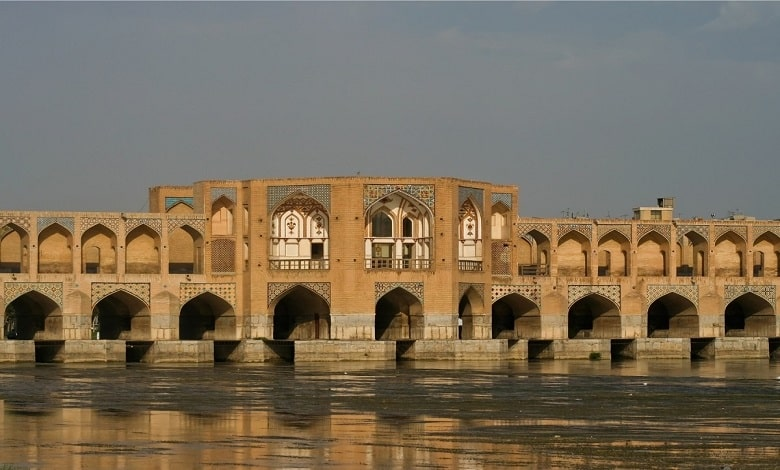
\includegraphics[width=\textwidth]{images/Near_set2.jpg}
        \caption{تصویر \lr{Near} (پل)}
    \end{subfigure}
    \hfill
    \begin{subfigure}{0.48\textwidth}
        \centering
        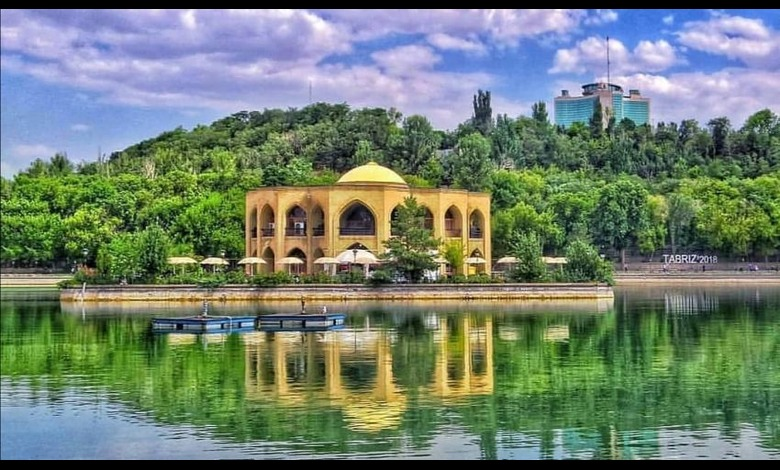
\includegraphics[width=\textwidth]{images/Far_set2.jpg}
        \caption{تصویر \lr{Far} (منظره)}
    \end{subfigure}
    \caption{تصاویر ورودی خام برای مجموعه‌های اول و دوم}
    \label{fig:input_images}
\end{figure}